\documentclass[11pt,a4paper]{article}
\usepackage[margin=2.6cm]{geometry}
\usepackage[T1]{fontenc}
\usepackage{lmodern}
\usepackage[letterspace=180]{microtype}
\usepackage{booktabs}
\usepackage{amsmath}
\usepackage{parskip}
\usepackage{xcolor}
\usepackage{tikz}
\usetikzlibrary{shapes.geometric,arrows.meta,positioning}
\usepackage[most]{tcolorbox}
\usepackage{titlesec}
\usepackage{caption}
\usepackage{graphicx}

\definecolor{bcnavy}{RGB}{24,38,68}
\definecolor{bcgold}{RGB}{198,160,74}
\definecolor{bcteal}{RGB}{23,110,120}
\definecolor{bcgrey}{RGB}{95,95,95}
\definecolor{bcred}{RGB}{160,60,50}

\titleformat{\section}{\bfseries\large\color{bcnavy}}{\thesection.}{0.6em}{}
\titleformat{\subsection}{\bfseries\color{bcteal}}{}{0em}{}
\captionsetup{font={footnotesize},labelformat=empty,textfont={color=bcgrey}}
\newcommand{\oneline}[1]{\begin{quote}\itshape\color{bcteal}Say it in one line:
``#1''\end{quote}}

\begin{document}

% ---------------------------------------------------------------- cover
\begin{titlepage}
\centering
\vspace*{3.2cm}

\includegraphics[width=5cm]{bc_logo.pdf}

\vspace{1.6cm}
{\color{bcnavy}\rule{7cm}{0.6pt}}

\vspace{0.9cm}
{\LARGE\bfseries\color{bcnavy} The Evolution of\\[0.15cm] Bayesian Capital\par}
\vspace{0.35cm}
{\large\color{bcnavy} Plain-language edition --- the story of how the company
got here,\\ told simply enough to explain to anyone\par}

\vspace{0.9cm}
{\color{bcgold}\rule{7cm}{1.0pt}}

\vspace{1.5cm}
{\bfseries Bayesian Capital}\\[0.2cm]
{\color{bcgrey} Systematic Trading Research}\\[0.9cm]
{\itshape\color{bcgrey} Internal document --- strictly confidential}\\[0.3cm]
{\color{bcgrey} 25 August 2026}
\vfill
\end{titlepage}

% ---------------------------------------------------------------- header
\begin{center}
{\Large\bfseries\color{bcnavy} The Evolution of Bayesian Capital}\\[0.15cm]
{\color{bcnavy} the plain-language edition}\\[0.25cm]
{\small\color{bcgrey} Bayesian Capital --- Systematic Trading Research
\;$\bullet$\; nine stocks: TSM $\cdot$ VRT $\cdot$ VST $\cdot$ RKLB $\cdot$ MU
$\cdot$ GM $\cdot$ VLO $\cdot$ CF $\cdot$ MRVL}
\end{center}
\vspace{0.1cm}
{\color{bcnavy}\hrule height 0.8pt}
\vspace{0.4cm}

\section{The whole story in one page}

\begin{center}
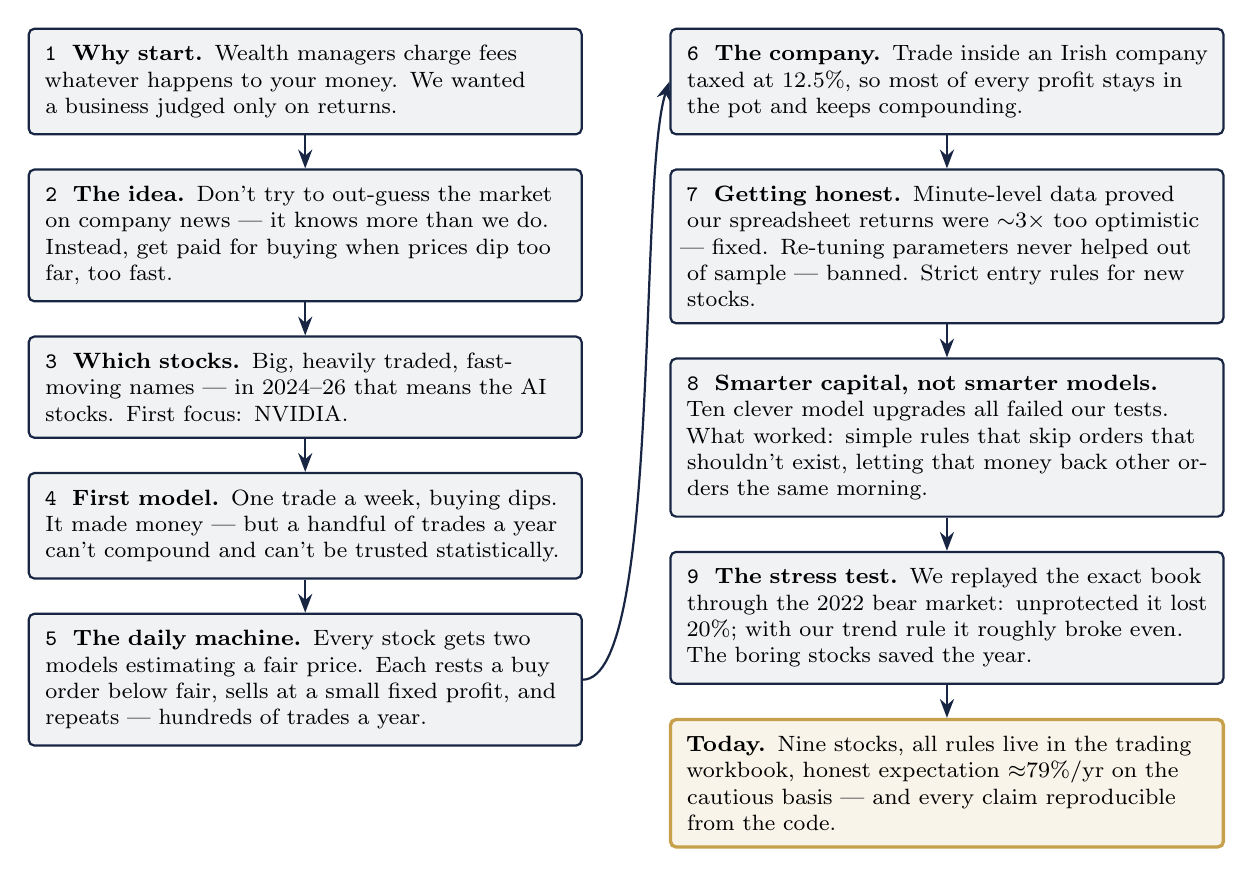
\begin{tikzpicture}[
  st/.style={rectangle, rounded corners=2pt, draw=bcnavy, thick, fill=bcnavy!6,
             text width=6.6cm, align=left, font=\footnotesize, inner sep=6pt},
  fin/.style={rectangle, rounded corners=2pt, draw=bcgold, very thick, fill=bcgold!12,
              text width=6.6cm, align=left, font=\footnotesize, inner sep=6pt},
  arr/.style={-{Stealth[length=2.4mm]}, thick, bcnavy},
  node distance=0.42cm]

\node[st] (s1) {{\tt 1 } \textbf{Why start.} Wealth managers charge fees
whatever happens to your money. We wanted a business judged only on returns.};
\node[st, below=of s1] (s2) {{\tt 2 } \textbf{The idea.} Don't try to
out-guess the market on company news --- it knows more than we do. Instead,
get paid for buying when prices dip too far, too fast.};
\node[st, below=of s2] (s3) {{\tt 3 } \textbf{Which stocks.} Big, heavily
traded, fast-moving names --- in 2024--26 that means the AI stocks. First
focus: NVIDIA.};
\node[st, below=of s3] (s4) {{\tt 4 } \textbf{First model.} One trade a week,
buying dips. It made money --- but a handful of trades a year can't compound
and can't be trusted statistically.};
\node[st, below=of s4] (s5) {{\tt 5 } \textbf{The daily machine.} Every stock
gets two models estimating a fair price. Each rests a buy order below fair,
sells at a small fixed profit, and repeats --- hundreds of trades a year.};
\node[st, right=1.1cm of s1] (s6) {{\tt 6 } \textbf{The company.} Trade
inside an Irish company taxed at 12.5\%, so most of every profit stays in the
pot and keeps compounding.};
\node[st, below=of s6] (s7) {{\tt 7 } \textbf{Getting honest.} Minute-level
data proved our spreadsheet returns were $\sim$3$\times$ too optimistic ---
fixed. Re-tuning parameters never helped out of sample --- banned. Strict
entry rules for new stocks.};
\node[st, below=of s7] (s8) {{\tt 8 } \textbf{Smarter capital, not smarter
models.} Ten clever model upgrades all failed our tests. What worked: simple
rules that skip orders that shouldn't exist, letting that money back other
orders the same morning.};
\node[st, below=of s8] (s9) {{\tt 9 } \textbf{The stress test.} We replayed
the exact book through the 2022 bear market: unprotected it lost 20\%; with
our trend rule it roughly broke even. The boring stocks saved the year.};
\node[fin, below=of s9] (s10) {\textbf{Today.} Nine stocks, all rules live in
the trading workbook, honest expectation $\approx$79\%/yr on the cautious
basis --- and every claim reproducible from the code.};

\draw[arr] (s1) -- (s2);
\draw[arr] (s2) -- (s3);
\draw[arr] (s3) -- (s4);
\draw[arr] (s4) -- (s5);
\draw[arr] (s5.east) .. controls +(1.0,0) and +(-0.4,-1.2) .. (s6.west);
\draw[arr] (s6) -- (s7);
\draw[arr] (s7) -- (s8);
\draw[arr] (s8) -- (s9);
\draw[arr] (s9) -- (s10);
\end{tikzpicture}
\end{center}

\section{Why start}

Most wealth management is paid through fees: a percentage of your assets,
every year, whatever happens. The provider does fine whether you do or not.
Bayesian Capital started from irritation with that model and one conviction:
build something judged \emph{only} on returns, where the person running the
money and the person owning it are the same.

\oneline{The industry is paid on fees; we wanted to be paid on returns.}

\section{The idea: get paid for other people's panic}

Two honest admissions came first. We can't out-research the market on
fundamentals --- thousands of professionals see every earnings report before
we do. And we don't have the technology for high-speed trading or options.
What's left? \textbf{Prices overshoot.} On volatile stocks, ordinary days
include moments of panic where the price dips several percent and bounces
back within hours. If you place a \emph{limit order} --- a standing instruction
to buy only at your chosen low price --- you get paid for being the calm buyer
in someone else's panic. No forecasting, no speed. Just discipline, patience,
and doing it hundreds of times a year.

\oneline{We don't predict stocks; we get paid a small premium, very often,
for buying dips that usually bounce.}

\section{Which stocks}

The strategy needs stocks that are \textbf{big and heavily traded} (so our
orders fill at fair prices) and \textbf{volatile} (so the dips are deep enough
to pay for the round trip). In this market that pointed straight at the AI
complex --- chipmakers, AI infrastructure, power --- with NVIDIA as the
original centrepiece. We knew this concentrated us in one theme; managing
that risk came later, deliberately.

\oneline{We fish where the fish are: liquid, volatile AI names.}

\section{The first model: right idea, wrong speed}

The first system traded \textbf{once a week}: buy a dip in NVIDIA or
Broadcom, sell at a target, repeat. The returns were strong --- but a dozen
trades a year has two fatal problems. You can't compound quickly, and you
can't tell skill from luck on so few trades. The fix wasn't a better formula;
it was a faster clock.

\oneline{The weekly model proved the idea but starved it --- we needed far
more trades.}

\section{The daily machine}

The system that trades today: each stock has \textbf{two models} estimating
what it's currently worth. One is a \emph{learning trend model} (it updates
its estimate of the stock's level and direction a little every day --- the
``Bayesian'' in our name). The other is a \emph{mean-reversion model} (it
assumes the price gets pulled back toward its recent average). Every morning,
each model places a buy order a safety margin \emph{below} its fair-price
estimate --- the margin scales with how wild the stock has been. When a dip
fills the order, we sell at a fixed few-percent profit target, then go again.
A position that goes wrong is sold after 50 days, no debate. Hundreds of
small wins a year, recycled --- \textbf{turnover is the engine}.

\oneline{Two fair-value models per stock, buy orders parked below fair,
quick fixed profits, hundreds of times a year.}

\section{The company: keeping the compounding}

Compounding only works if profits stay in the pot. Realised trading gains
inside an \textbf{Irish trading company are taxed at 12.5\%} --- so 87.5 cents
of every euro earned goes straight back to work, versus roughly half under
personal tax rates. Over years, that difference decides whether compounding
snowballs or stalls. The company isn't paperwork; it's part of the maths.

\oneline{At 12.5\% tax, seven-eighths of every profit goes back into the
machine.}

\section{Getting honest}

Growing from two stocks to a book forced the hard question: \emph{which of
our numbers are real?} Three disciplines came out of it.

\textbf{Verified fills.} Our spreadsheet counted a same-day buy-and-sell
whenever the day's low touched our buy price and the high touched our target.
But daily data can't tell you which happened \emph{first}. Minute-by-minute
data proved the spreadsheet was roughly \textbf{three times too optimistic}.
Since then, no trade counts unless the minute data proves the buy happened
before the sell.

\textbf{No re-tuning.} Every attempt to re-optimise the model's parameters on
recent data made things \emph{worse} on data it hadn't seen --- dozens of
tests, same answer. Parameters were frozen. (One genuine formula bug --- the
mean-reversion model was measuring trend instead of noise --- was found and
fixed. Bugs get fixed; parameters don't get chased.)

\textbf{Entry rules for stocks.} A stock joins the book only by passing fixed
gates: clean verifiable data; classification (AI-linked stocks must promise
50\%+ a year, genuinely unrelated ones 30\%+); the model must work on data it
wasn't fitted to; and the stock must make the \emph{book} better, not just
itself. These gates admitted four stocks and rejected ten --- including famous
names like NVIDIA and Tesla, on numbers, not opinions.

\oneline{We measure honestly, never re-tune, and let fixed rules --- not
excitement --- decide what we trade.}

\section{Smarter capital, not smarter models}

With parameters frozen, we spent weeks trying to make the models cleverer:
better volatility forecasts, market-regime detectors, adaptive profit
targets, stop-losses, and a more sophisticated mean-reversion model
(Schwartz--Smith). \textbf{All ten failed our tests} --- each one damaged the
simple harvest it tried to improve.

What worked was different: moving \emph{capital} more intelligently. Our
workbook pools each morning's cash across whichever stocks are free to trade
--- so if a stock is told to stand down, its money isn't idle, it backs the
other orders that same morning. Three ``stand down'' rules passed every test
and are now live:

\begin{itemize}
\item \textbf{The trend rule (200-day average):} don't buy dips in a stock
trading below its own 200-day average price --- that's not a dip, that's a
downtrend. This is our bear-market protection.
\item \textbf{The record-high rule:} never place an order whose profit target
would need the stock to hit a new all-time high to get out.
\item \textbf{The pre-market rule:} at 9am, cancel any order more than 4\%
below where the stock is already trading pre-market --- those orders almost
never fill, and the rare fills are bad news. Worth about ten percentage
points a year to the book.
\end{itemize}

The lesson, learned ten times: \textbf{changes that give the model new
information and simply cancel bad orders can win; changes that second-guess
how the model trades always lose.} And a cancelled order is never re-priced.

\oneline{Ten clever model upgrades failed; three simple `skip this order'
rules, backed by pooled capital, are what actually worked.}

\section{The stress test}

Everything above was measured in a bull market. So we obtained minute-level
data for 2021--2023 and replayed today's exact book through the
\textbf{2022 bear market} --- a year our AI names fell 40--80\%. Unprotected,
the book lost about 20\% (painful, survivable). With the trend rule active it
lost about 1\% --- because the money that stopped chasing falling AI stocks
was automatically redeployed into the ``boring'' stocks (GM, Valero, CF),
which had a great year. The diversifiers, admitted for exactly this scenario,
earned their place.

One more honesty upgrade closed the loop: our sell orders are limit orders,
so when a stock jumps \emph{over} our target overnight, we get filled at the
better opening price. The model wasn't counting that --- reality pays about
20 percentage points a year more at book level than our cautious models
claimed. On the careful planning basis the book targets \textbf{roughly
79\% a year}; the fuller simulation of the live setup measures around 106\%.

\oneline{We replayed 2022: unprotected minus twenty, with our rules roughly
flat --- and our real-world executions are better than our models assumed.}

\section{If you're asked\ldots}

\begin{tcolorbox}[colback=bcnavy!5, colframe=bcnavy, boxrule=0.8pt,
  title={\bfseries Five questions you should be ready for}, coltitle=white]
\textbf{``What's your edge?''} --- Patience and turnover, not prediction. We
supply liquidity into short-lived panics in volatile stocks and collect a
small premium hundreds of times a year. Our process edge is honesty: verified
fills, frozen parameters, fixed admission gates.

\textbf{``How do you avoid overfitting?''} --- We fit on the first half of the
data, freeze everything, and only believe the second half. Re-tuning lost in
almost every test we ran, so parameters are frozen and only structural rules
that improve \emph{both} halves independently get adopted. Ten of thirteen
proposals died by that rule.

\textbf{``What happens in a crash?''} --- We replayed our exact book through
2022: minus 20\% unprotected, roughly flat with the 200-day trend rule that
now runs live, because gated capital rotates into the non-AI names. The known
weak spot is a very fast crash, which the trend rule is too slow to see ---
that's a bounded, understood risk.

\textbf{``Why these nine stocks?''} --- They passed fixed gates: liquid,
volatile, verifiable data, model works out of sample, and each one made the
book better. We rejected NVIDIA, Tesla, Broadcom, AMD and others on the same
numbers --- the gates don't care about fame.

\textbf{``Why will it keep working?''} --- Volatility and panic aren't going
away, our stocks are chosen for exactly those traits, and the whole edifice
is re-checkable: every claim reproduces from code and data. And when the
regime changes, our protection was tested on a real bear market, not a
story.
\end{tcolorbox}

\vspace{0.4cm}
{\color{bcnavy}\hrule height 0.8pt}
\vspace{0.2cm}
{\footnotesize\color{bcgrey} Companion (technical) edition: \emph{The
Evolution of Bayesian Capital}, same date. Detailed sources: \emph{Verified
Book Ranking}; \emph{Book Admission Gates}; \emph{Three Volatility Overlays,
Tested and Rejected}; \emph{Bear-Market Protection for the Nine-Name Book};
\emph{The Pre-Market Rule}.}

\end{document}
